%% Figure 1: where the archives are (map) and what an orphan looks like (KBo 24.8, CTH 470).
%% Map: figures/make_archive_map.py (base map fetched, not in git). Fragment images:
%% figures/fetch_fragment_images.sh (not in git). Transliteration: TLHdig 0.4, KBo 24.8.
\providecolor{clay}{RGB}{176,74,46}
\newcommand{\hb}[1]{{\fontspec{Noto Sans Display}#1}}   % half brackets, missing in Termes
\newcommand{\hit}[1]{\textit{#1}}                         % Hittite and Akkadograms in italics
\begin{figure*}[!t]
  \centering
  %% Body of Figure 1 (map, photo, hand copy, transliteration); used by map_fragment_fig.tex and,
%% for the Word copy, by fig1_standalone.tex.
  \begin{minipage}[b]{0.49\linewidth}\centering
    \resizebox{\linewidth}{!}{% generated by figures/make_archive_map.py; do not edit
\begin{tikzpicture}
\node[anchor=south west, inner sep=0] at (0,0) {\includegraphics[width=7.7cm]{external/map_wide_colour_hl.png}};
\draw[gray!60, line width=0.3pt] (0,0) rectangle (7.7,5.133);
\filldraw[fill=clay, draw=white, line width=0.35pt] (4.421,3.562) rectangle (4.591,3.732);
\filldraw[fill=clay, draw=white, line width=0.35pt] (4.784,3.708) rectangle (4.914,3.838);
\filldraw[fill=clay, draw=white, line width=0.35pt] (5.102,3.679) rectangle (5.202,3.779);
\filldraw[fill=clay, draw=white, line width=0.35pt] (5.481,3.301) rectangle (5.581,3.401);
\filldraw[fill=clay, draw=white, line width=0.35pt] (5.793,3.167) rectangle (5.867,3.242);
\filldraw[fill=white, draw=gray!50, line width=0.2pt, rounded corners=1pt] (0.1,0.1) rectangle (1.7200000000000002,1.120);
\node[anchor=north west, font=\fontsize{4}{4.8}\selectfont\bfseries, inner sep=1pt] at (0.14,1.100) {Tablets and fragments};
\filldraw[fill=clay, draw=white, line width=0.35pt] (0.165,0.735) rectangle (0.335,0.905);
\node[anchor=west, font=\fontsize{4}{4.8}\selectfont, inner sep=1pt] at (0.4,0.820) {over 10{,}000};
\filldraw[fill=clay, draw=white, line width=0.35pt] (0.185,0.555) rectangle (0.315,0.685);
\node[anchor=west, font=\fontsize{4}{4.8}\selectfont, inner sep=1pt] at (0.4,0.620) {1{,}000--10{,}000};
\filldraw[fill=clay, draw=white, line width=0.35pt] (0.200,0.370) rectangle (0.300,0.470);
\node[anchor=west, font=\fontsize{4}{4.8}\selectfont, inner sep=1pt] at (0.4,0.420) {100--1{,}000};
\filldraw[fill=clay, draw=white, line width=0.35pt] (0.212,0.183) rectangle (0.287,0.258);
\node[anchor=west, font=\fontsize{4}{4.8}\selectfont, inner sep=1pt] at (0.4,0.220) {under 100};
\node[anchor=south east, font=\fontsize{4}{4.8}\selectfont, text=gray!70!black, fill=white, inner sep=1.5pt] at (7.7,0) {Base map: Cammarosano, CC BY-SA};
\end{tikzpicture}
}\\[2pt]
    {\footnotesize (a)}
  \end{minipage}\hfill
  \begin{minipage}[b]{0.20\linewidth}\centering
    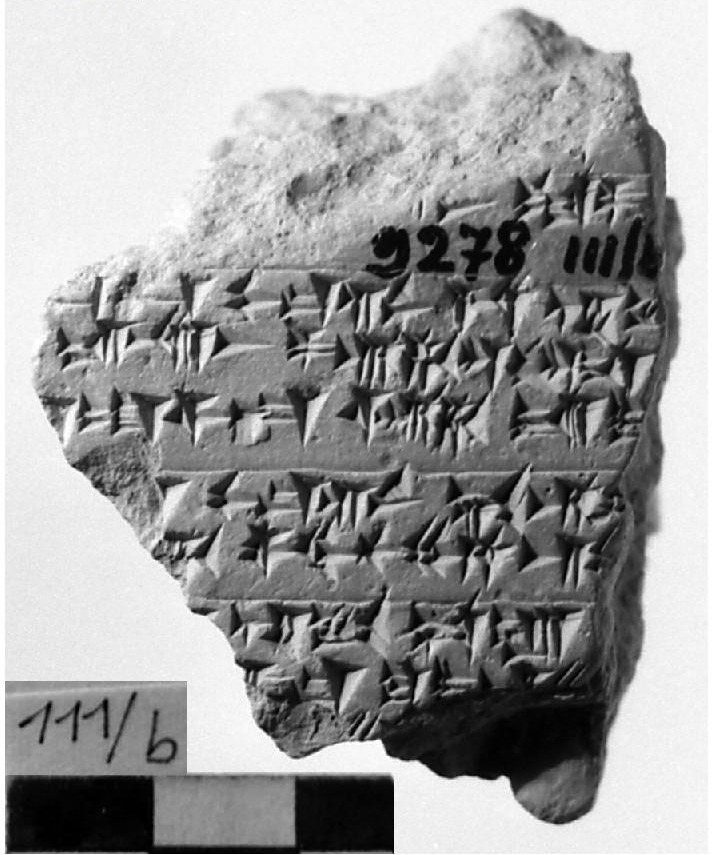
\includegraphics[height=5.1cm]{external/KBo_24_8_photo.jpg}\\[2pt]
    {\footnotesize (b)}
  \end{minipage}\hfill
  \begin{minipage}[b]{0.27\linewidth}\centering
    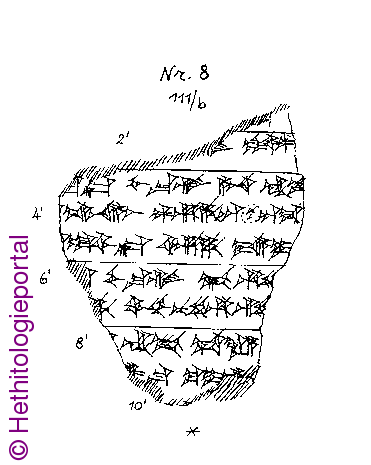
\includegraphics[height=5.1cm]{external/KBo_24_8_handcopy.png}\\[2pt]
    {\footnotesize (c)}
  \end{minipage}\\[6pt]
  \begin{minipage}{\linewidth}\centering\small
    \begin{tabular}{@{}r@{\hspace{6pt}}l@{}}% generated by figures/make_fragment_translit.py; do not edit
1$'$ & [\ensuremath{\circ}\,\ensuremath{\circ}\,\ensuremath{\circ}\,\ensuremath{\circ}\,\ensuremath{\circ}\,\ensuremath{\circ}\,\ensuremath{\circ}\,\ensuremath{\circ}\,\ensuremath{\circ}\,\ensuremath{\circ}\,\ensuremath{\circ}]x[\ensuremath{\circ}] \\
2$'$ & [\ensuremath{\circ}\,\ensuremath{\circ}\,\ensuremath{\circ}\,\ensuremath{\circ}\,\ensuremath{\circ}\,\{MUNUS\}ŠU.G]I EGIR-\hit{pa} [\ensuremath{\circ}\,\ensuremath{\circ}] \\
3$'$ & [\ensuremath{\circ}]x-\hit{kán} \{MUNUS\}ŠU.GI \hit{A-NA} EN SIS[KUR \ensuremath{\circ}\,\ensuremath{\circ}\,\ensuremath{\circ}] \\
4$'$ & [\ensuremath{\circ}]x \hit{iš-na-a-aš pa-tal-ḫa-an} (erasure) \hit{an-da} [\ensuremath{\circ}] \\
5$'$ & [\ensuremath{\circ}]x-\hit{at-ši-kán ar-ḫa da-a-i} [\ensuremath{\circ}\,\ensuremath{\circ}] \\
\end{tabular}\hspace{2em}%
    \begin{tabular}{@{}r@{\hspace{6pt}}l@{}}% generated by figures/make_fragment_translit.py; do not edit
6$'$ & [\ensuremath{\circ}]x \{MUNUS\}ŠU.GI \{DUG\}\hit{ḫu-p}[\hit{u-} \ensuremath{\circ}\,\ensuremath{\circ}\,\ensuremath{\circ}\,\ensuremath{\circ}] \\
7$'$ & [\hit{ar-ḫ}]\hit{a wa-aḫ-nu-uz-zi} [\ensuremath{\circ}\,\ensuremath{\circ}\,\ensuremath{\circ}\,\ensuremath{\circ}\,\ensuremath{\circ}] \\
8$'$ & [\ensuremath{\circ}\,\ensuremath{\circ}]x EN SISKUR \hit{ša-ra-a} [\ensuremath{\circ}\,\ensuremath{\circ}\,\ensuremath{\circ}] \\
9$'$ & [\ensuremath{\circ}\,\ensuremath{\circ}\,U]DU-\hit{ŠU ku-i-}\hb{⸢}\hit{e}\hb{⸣}\hit{-e}[\hit{š} \ensuremath{\circ}\,\ensuremath{\circ}\,\ensuremath{\circ}\,\ensuremath{\circ}] \\
10$'$ & [\ensuremath{\circ}\,\ensuremath{\circ}\,\ensuremath{\circ}\,\ensuremath{\circ}\,\ensuremath{\circ}]x x[\ensuremath{\circ}\,\ensuremath{\circ}\,\ensuremath{\circ}\,\ensuremath{\circ}\,\ensuremath{\circ}] \\
\end{tabular}\\[3pt]
    {\footnotesize (d)}
  \end{minipage}

  \caption{The archives and one of their orphans. (a) The Hittite archives on the map of
    \citet{cammarosano2017map}; squares show the number of tablets and fragments
    \citep{hoffner2024grammar,rieken2019kayalipinar}. (b) Photograph, (c) hand copy and (d)
    TLHdig transliteration of the orphan KBo 24.8 (\CTH{470}); circles mark lost signs,
    estimated from the line layout in TLHdig. The method places it with the Luwian rituals.}
  \label{fig:fragment}
\end{figure*}
